% Chapter 3 from the thesis template file
%   that contains an example table and figure.

%Chapter 3: Background
%1) Introduction paragraph summarizing the flow/content/structure of the Background chapter
%2) Radiometer Basics
%	a) Power Detection
%	b) Integration and filtering
%	c) Metrics
%		i) Sensitivity
%		ii) Stability
%	d) Implementation
%3) Software Defined Radio Basics
%	a) High-level figure of the components of a generic SDR.
%	b) SDR Operation
%	c) GNURadio Operation
%4) Software Defined Radio Development Platform (i.e. your specific platform)
%	a) Hardware (i.e. N200)
%	b) Software (i.e. GNU Radio)  

\chapter{BACKGROUND}\label{ch:background}

To develop a software defined radiometer, it is important to study how a traditional radiometer works, how a software defined radio works and the development tools used to develop a software defined radiometer.  This chapter will give background information on the operation of a traditional radiometer and on a software defined radio.  We will begin by looking at the major components of a radiometer and how it measures power.  Next we will look at the metrics used to measure performance of a traditional radiometer.  Finally, we will also give information on the development tools used to build a software defined radiometer.  

%We begin with an overview of a traditional radiometer and how this type of radiometer works.  This is followed by high level examination of a software defined radio.  Finally we will discuss the hardware and software to be used for our development of a software defined radiometer.

\section{Radiometer Basics}\label{rad_basics}
A radiometer is a device that is designed to measure thermal electromagnetic emission by a material media[\cite{ulaby}.  The amount of noise that is generated by the material media is due to the thermal agitation of the charge carriers, usually the electrons, which is directly correlated to the physical temperature of the source [\cite{Nyquist1928thermal}].  Because of this correlation, the amount of noise received is called the noise temperature and it is measured in Kelvin. 

In all radiometers there are six stages that is common in all radiometers.  They are:

\begin{enumerate}
\item Source (antenna or $T_{A}$)
\item Amplification (Gain or $G$),
\item Bandwidth ($\beta$),
\item Power detection ($X^{2}$),
\item Integration ($\tau$),
\item Output (Voltage, rQ or Kelvin).
\end{enumerate}

Figure \ref{trad_radiometer} shows each stage, beginning with our source, which is often an antenna.  Gain is the amplification done to the signal so that it is easier to measure changes in the source.  Bandwidth is the range of frequencies that are being observed.  Bandwidth may be set by filters or by hardware limitations. 

Power detection and measurement is done using a square-law detector and will be discussed more in section \ref{pwr_measurement}.  A square-law detector takes the input RF signal and produces a voltage that is proportional to the square of the voltage[\cite{Leinweber}].  

Because this voltage signal is often noisy, an integrator is used to smooth our signal and improve our sensitivity. This is implemented in hardware with a low pass filter and it removes the high frequency components from the signal.  Finally the output is the total power information and is a voltage output from the square-law detector and may be calibrated as a noise temperature measured in Kelvin.

{\begin{figure}[h!tb] 
\centering
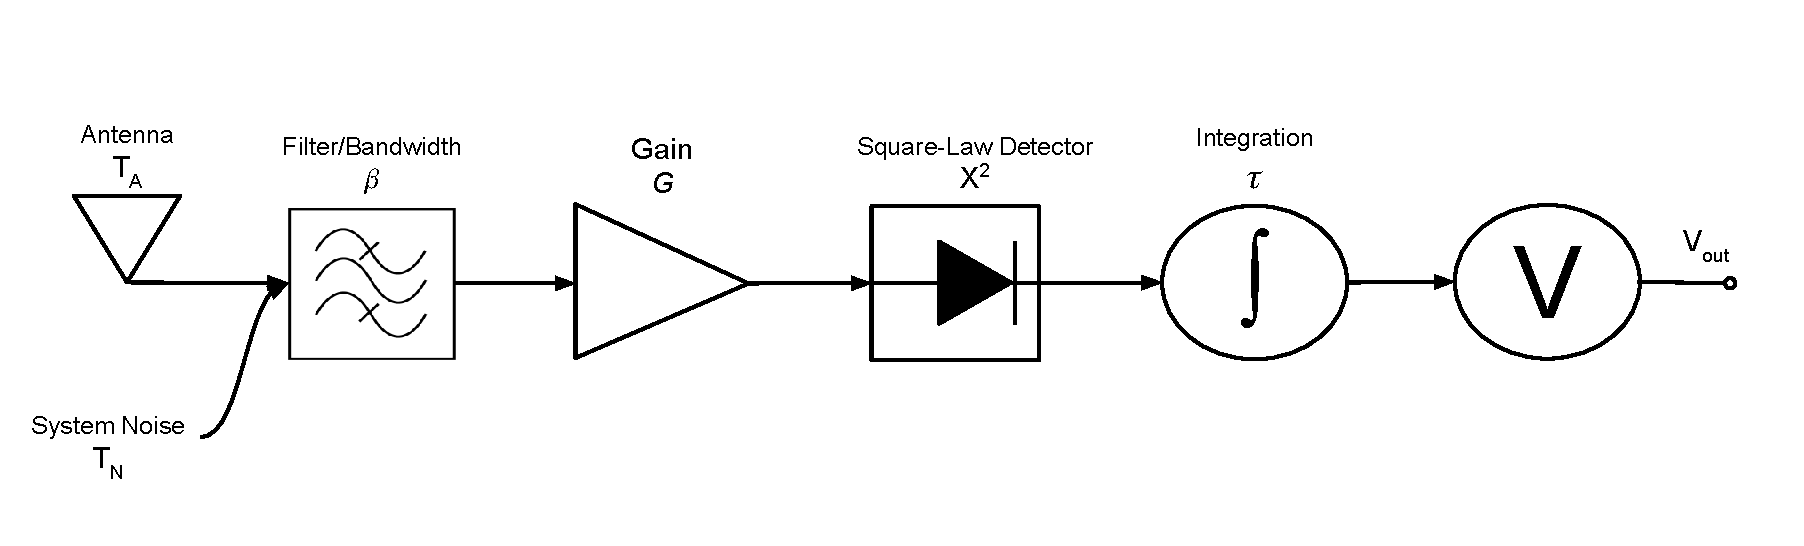
\includegraphics[width=\textwidth]{Images/Traditional_Radiometer.pdf}
\isucaption{A total power radiometer block diagram}
\label{trad_radiometer}
\end{figure}
}

A non-physical object that is present in all radiometers is system noise, represented as $T_{N}$.  System noise is noise that is generated from within the radiometer due to thermal agitation.  A radiometer is designed to reduce the system noise as much as possible by using low-loss components and amplifiers that are low noise such as Low Noise Amplifiers (LNA). 

In the next section, how a radiometer measures power will be examined.  This is an important function of the radiometer as it is the primary function of the radiometer.

\subsection{Power Measurement}\label{pwr_measurement}

%To measure power in a radiometer, several factors are taken into consideration.  To begin with we have the noise signal coming from the antenna.  Our antenna is assumed to be looking at our target of interest and it is assumed that we can relate the antenna noise to the noise from the source.  It is often easier to refer to this noise as the brightness temperature.  Therefore, the brightness temperature of the source can be related to the brightness temperature at the antenna.  We will refer to this brightness temperature as $T_{A}$.  

The power output from a radiometer is determined from the gain ($G$), the bandwidth ($\beta$), and from the source ($T_{A}$).  Equation \ref{eq:power_rad_eq} gives the total power, in watts, of an ideal radiometer by taking our gain, bandwidth and source and multiplying this by the Boltzmann constant, known as \textit{k} and has a known value shown in equation \ref{eq:boltzmann} .

\begin{equation} \label{eq:power_rad_eq}
P=k*\beta*G*(T_{A}) (watts)
\end{equation}

\begin{equation} \label{eq:boltzmann}
k = 1.3806488 x 10^{-23} J/K
\end{equation}

An ideal radiometer is one in which none of the components contribute any additional noise to the system.  Since an ideal radiometer does not exist, this additional noise must be accounted for.  Figure \ref{rad_basics} shows this additional noise as $T_{N}$ and represents the system noise.  The system noise is added to the source or antenna noise and this results in equation \ref{eq:final_power}.

\begin{equation} \label{eq:final_power}
P=k*\beta*G*(T_{A}+T_{N}) (watts)
\end{equation}

The gain, $G$ and the bandwidth $\beta$ are two variables that can be altered in this design of a traditional radiometer.  When possible, the gain is increased as much as possible.  The limitation is that we desire to have the system noise as low as possible.  Increasing the gain, will increase the system noise contributed.  It is also desirable to increase the bandwidth as much as possible.  The limitation with bandwidth may be due to hardware or may be due to the properties of the range of frequencies we are observing.  Different frequencies have different properties for the objects we are observing.  Other frequencies are used for other functions, such as radio communications, and this interferes with the radiometer.  

%Figure \ref{trad_radiometer} showed a typical radiometer and was discussed in the previous section.  However, power detection and the associated voltage output has not been discussed.  Power detection is accomplished typically with a square-law detector and this output is often run through an integrator to smooth the output[\cite{Leinweber}].  Finally we have the output which is a voltage represented as V$_{out}$.  This results in equation~\ref{eq:vout_1}.

%\begin{equation} \label{eq:vout_1}
%V_{OUT}=c*(T_A+T_N)*G
%\end{equation}

%Here V$_{OUT}$ is shown by the addition of both the noise from the system T$_N$ and the noise from the antenna, T$_A$ and multiplied by the gain in the system, $G$ [\cite{skou}].  A constant factor $c$ is useful for when we are looking at a radiometer like a Dicke radiometer in which the value of $c$ is $\frac{1}{2}$.  In most applications outside of a Dicke radiometer, $c$ is 1 and can be ignored.  

%The voltage output from this radiometer is then either measured or may also be sampled by an analog to digital converter.  This voltage then represents the total power measured by the radiometer, however this measurement is not calibrated.

%\subsection{Integration and filtering}\label{int_filt}

%Filtering with a traditional radiometer is usually accomplished by using mechanical filters.  Often these are band-pass filters that limit the bandwidth that the radiometer sees.  Other filters, such as a low pass filter are also used, but usually to smooth out the output from the square law detector.  Another item used to help smooth out the signal from the square law detector is an integrator.

%In a traditional radiometer, we can integrate by using a simple RC circuit, which consists of a resistor and capacitor.  To begin, we will examine how a RC filter is analogous to an integrator where the R and C values determine our time constant and our integration time for the filter[\cite{Aitken}].  We know a RC filter is analogous to an integrator by looking at equation \ref{eq:rc_int}.  

%\begin{equation}\label{eq:rc_int}
%\frac{1}{RC}\int{V_idt}
%\end{equation}

%To begin with, we look at what an analog RC filter looks like. 

%{\begin{figure}[h!tb] 
%\centering
%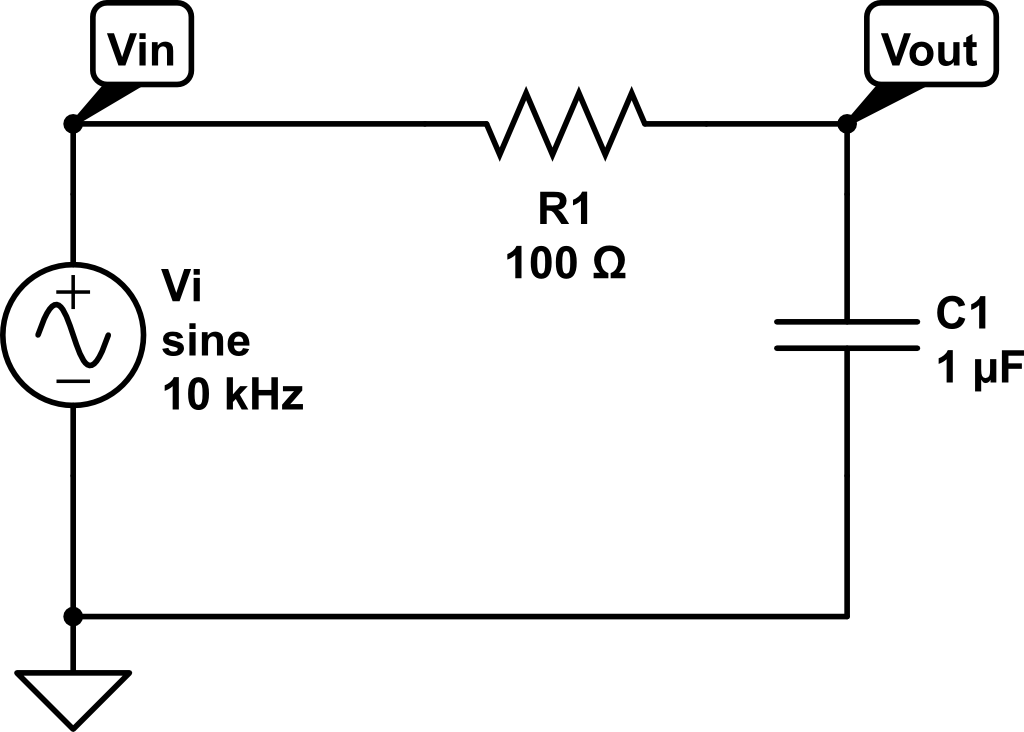
\includegraphics[width=10cm]{Images/rc-circuit.png}
%\isucaption{A simple RC circuit}
%\label{rc_circuit}
%\end{figure}
%}

%This circuit can be represented by equation \ref{eq:rc_circuit_eq}.

%\begin{equation}\label{eq:rc_circuit_eq}
%\frac{V_{in}-V_{out}}{R}=C\frac{dV_{out}}{dt}
%\end{equation}

%For the cutoff frequency of a RC circuit, we know that it has the relationship shown in equation \ref{RC_relationship}.

%\begin{equation}\label{RC_relationship}
%f_c=\frac{\sqrt{3}}{2\pi RC}\rightarrow RC=\frac{\sqrt{3}}{2\pi f_c}
%\end{equation}

%The $RC$ term gives us our time constant of the circuit and can be used to calculate out our coefficients. 

\subsection{RF Front End}
As discussed in section \ref{pwr_measurement}, gain plays an important role in the power received by the radiometer.  This can be seen by looking at equation \ref{eq:final_power}.  As we will soon discuss in section \ref{performance_metrics}, it also plays a key role in a radiometers sensitivity as well.  It is also our largest source of system noise.  Ideally, we want as much gain as possible, but we want our system noise contributed as low as possible.  A Low Noise Amplifier (LNA) is designed to give as much gain as possible while keeping the noise it contributes as low as possible.  

A method to increase gain, but keep our noised added to the system low, is to daisy chain two or more LNAs together.  This results in the gain of each LNA to sum up to a desired total gain.  However, the system noise does not sum up.  The relationship between the noise factor ($F$) and the gain ($G$) can be seen in equation \ref{noise_factor}.  

\begin{equation}\label{noise_factor}
F=F_1+\frac{F_2-1}{G_1}+\frac{F_3-1}{G_1 G_2}+\frac{F_4-1}{G_1 G_2 G_3}+\cdots +\frac{F_n-1}{G_1 G_2 G_3 \cdots G_{n-1}}
\end{equation}

The first LNA in the chain has the largest impact on the amount of system noise that is contributed to the system.  While the additional LNAs do contribute to the system noise, it is at a fraction of the first LNA.  For this reason we use a LNA that has a very low noise factor, but does not provide a lot of gain.  However, we then add additional LNAs after the first LNA that often has higher gain values.  This will mean that they also have a higher noise factor, but their noise contribution is not as much due to equation \ref{noise_factor}.

%The RF front end plays an important role in the radiometer because the LNAs used in the front end have a large impact on the system noise generated by the radiometer itself.  A traditional radiometer utilizes both amplification through the LNAs and also includes filtering to the desired bandwidth.  A SDR radiometer does not require the filters as we are able to create these in software, however the amplification stages need to remain.  

%{\begin{figure}[h!tb] 
%\centering
%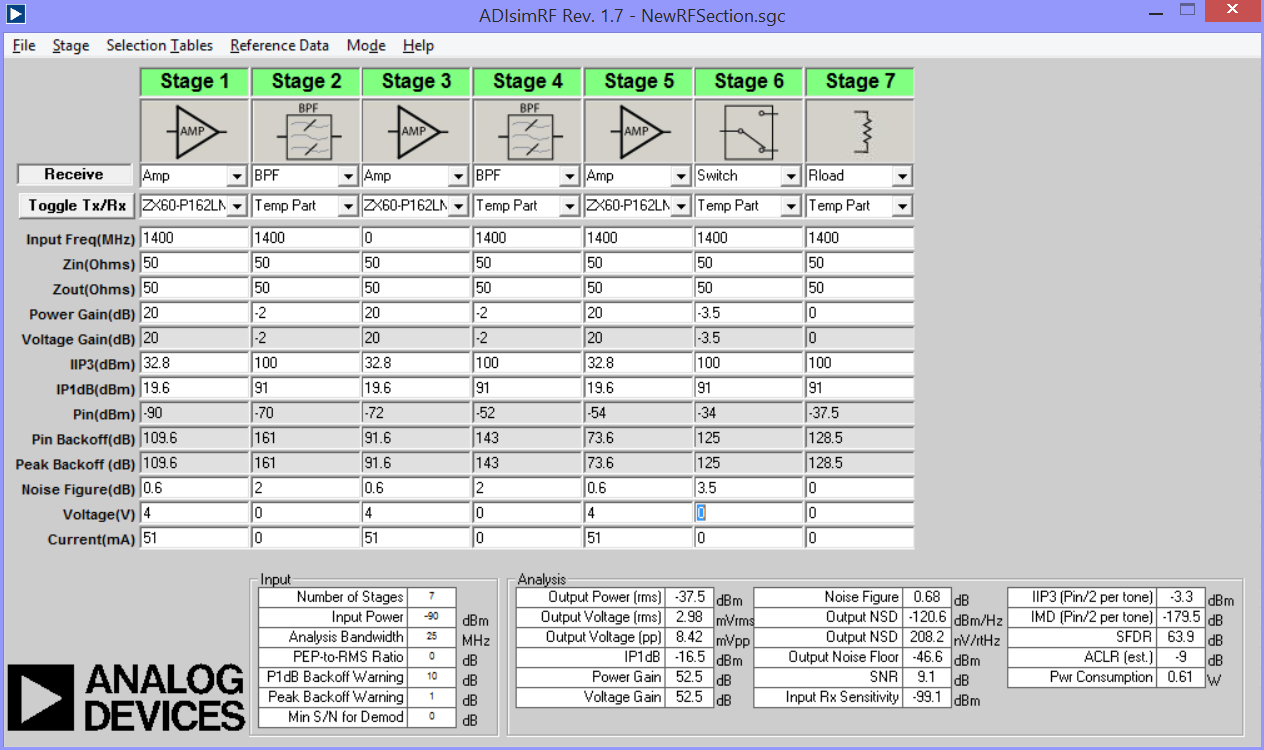
\includegraphics[width=0.8\linewidth]{Images/RF_Front_end.png}
%\isucaption{The ADISIMRF program used to verify the design of the RF Front End}
%\label{ISU_Rad}
%\end{figure}
%}

%A typical RF front end uses a two to four stage Low Noise Amplifier (LNA) to amplifier the noise while keeping the noise contributed to the system as low as possible.  As with any radiometer, the first LNA is the most critical as it contributes the most to the overall system noise temperature.  For this reason a LNA that did not have a large gain but had a low noise figure is chosen. The second and third LNA has higher gain values at the cost of a higher noise figure, although not by much.  However, since they are further down the chain, they do not contribute as much to the total system noise.  


Equation \ref{noise_factor} shows us how the noise factor and gain of the amplifiers affect each other.  It can be shown that the first amplifier or first noise figure in the system contributes the most to the overall system noise figure.  Additional components contribute, but at a much lower contribution.

\subsection{Radiometer Performance Metrics}\label{performance_metrics}

Two criteria used to determine how well a radiometer performs are: 1) Sensitivity and 2) Stability.  These criteria determine the smallest amount of change in the noise temperature the radiometer can detect and the amount of error it has in its measurements.

\emph{Sensitivity}.  Sensitivity of a radiometer is the smallest amount of change in power that can be detected.  A radiometer must be able to differentiate noise from the antenna source and the system generated in the radiometer.  This noise is added to the signal and can not be separated from the signal.  Because this noise is added to the signal, the ability to determine a change in the signal while the noise signal is also present is key.  

To understand this, look at the example of where T$_{A}$ has a value of 200 K and T$_{N}$ has a value of 800 K.  Since T$_{N}$ is added to the antenna signal, we have a total noise temperature of 1,000 K.  This means to detect a change as small as 1 K, the difference between 1,000 K and 1,001 K needs to be measured.[\cite{skou}].

The ability of a radiometer to detect these small changes is the radiometer's sensitivity, or the standard deviation of the output signal from the radiometer.  This sensitivity is also referred to as the Noise Equivalent Delta ($\Delta$) Temperature or NE$\Delta$T and is shown in equation \ref{NEAT_EQ}. 

\begin{equation} \label{NEAT_EQ}
NE\Delta T=\frac{T_{A}+T_{N}}{\sqrt{\beta * \tau}} 
\end{equation}

The sensitivity of the radiometer is a function of the bandwidth, ($\beta$), of the incoming signal and the integration time, ($\tau$) used.  Since the sensitivity improves as the bandwidth increases, as much bandwidth that is possible is desired.  In a traditional radiometer, this bandwidth is often fixed and it is dependent on the band-pass filters used in the radiometer.  A longer integration time ($\tau$) will also help improve the sensitivity of the radiometer to a certain degree.[\cite{ulaby}]

\emph{Stability.}  The primary task of a radiometer is to measure power to within a certain degree of accuracy.  In order to accurately and precisely measure power to a high degree, a radiometer must take into account factors such as the system noise, the bandwidth of the signal and the stability of the system as a whole[\cite{Evans}]. 

Instabilities in a radiometer are due to fluctuations in the gain values in a Low Noise Amplifiers (LNAs) which are referred to as gain fluctuations.  Two factors cause gain fluctuations: voltage changes and the physical temperature of the LNA.  

The impact these gain fluctuations have in the system are shown in equation \ref{eq:rad_stability}.  Here, the change in the noise temperature due to gain fluctuations, $\Delta T_{G}$, is a result of the change in the gain, $\Delta G$ divided by our gain, $G$, and multiplied by our system noise, $T_{sys}$.  

\begin{equation} \label{eq:rad_stability}
\Delta T_G=T_{sys} \left(\frac{\Delta G}{G}\right)
\end{equation}

These gain fluctuations can be controlled by closely monitoring and controlling both the voltage and the temperature of the LNAs. However, this adds complexity to the radiometer which can be impractical in some cases.  Therefore, other types of radiometers have been developed to compensate for these fluctuations.  There are three common types of radiometers designed to adjust for gain fluctuations.  They are: Dicke radiometer, Noise injection radiometer, and Polarimetric or correlating radiometer.

The first type of radiometer used is the Dicke radiometer.  Figure \ref{dicke_radiometer} shows a block diagram of a Dicke radiometer which switches between the measurement of the source or antenna and a known reference source[\cite{Dicke}].  By referencing this reference source very quickly the Dicke radiometer can account for and greatly reduce gain fluctuations.  

{\begin{figure}[h!tb] 
\centering
\includegraphics[width=\textwidth]{Images/Dicke_block.png}
\isucaption{A block diagram of a Dicke radiometer}
\label{dicke_radiometer}
\end{figure}
}

While a Dicke radiometer greatly reduces the fluctuations seen in the gain of a radiometer and improves stability, it does so at the cost of not seeing the object of interest while it is referencing the known source.  Because of this, the overall sensitivity of the radiometer is decreased.

{\begin{figure}[h!tb] 
\centering
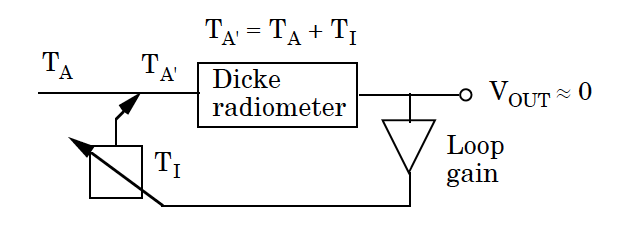
\includegraphics[width=\textwidth]{Images/NoiseInj_block.png}
\isucaption{A block diagram of a Noise Injection radiometer}
\label{NoiseInj_radiometer}
\end{figure}
}

A noise injection radiometer is a variation of the Dicke radiometer where a variable noise source is used and injected into the RF chain as seen in Figure \ref{NoiseInj_radiometer}.  The output of this noise source is then adjusted so the noise input plus the signal from the source is equal to the reference noise.  This completely eliminates gain fluctuations but, it increases the system noise which also reduces the sensitivity of the radiometer.

A polarimetric or correlating radiometer uses two polarized signals, referred to as vertical polarization (V-Pol) and horizontal polarization (H-Pol).  In order to accomplish this, an antenna with dual polarization is used [\cite{Fujimoto}].  Each polarized signal is then fed into the radiometer and correlated.  Because the noise signal of interest has polarization and the gain fluctuations does not, it can eliminate the gain fluctuations.  This reduces gain fluctuations and helps maintain the sensitivity of the radiometer but at the cost of adding complexity to the radiometer. A correlating radiometer requires two identical receivers, one for each polarization. 


%Stability and accuracy are additional problems that need to be considered when looking at the radiometer system.  To begin we can once again look at the power received equation \ref{eq:final_power}.

%As we look at this equation, we can see that if $k$, $\beta$, $G$, and $T_{N}$ are constant, then stability can be assured.  The Boltzman constant $k$ is a known constant and we can also assume that our bandwidth, $\beta$, will also remain constant.  Gain and the noise temperature however will vary.  

 
\section{Software Defined Radios Basics} 
A Software Defined Radio (SDR) is defined as a device that will digitize a received RF signal as soon as possible, and processes the digital representation of the signal with a computer, FPGA, or a dedicated System on Chip (SoC).  A canonical software defined radio architecture is one that consists of a power supply, antenna, analog to digital converter, and a processing unit to carry out the radio functions in software [\cite{Mitola1995}]. An ideal software defined radio block diagram is shown in figure \ref{ideal_sdr}.

{\begin{figure}[h!tb] 
\centering
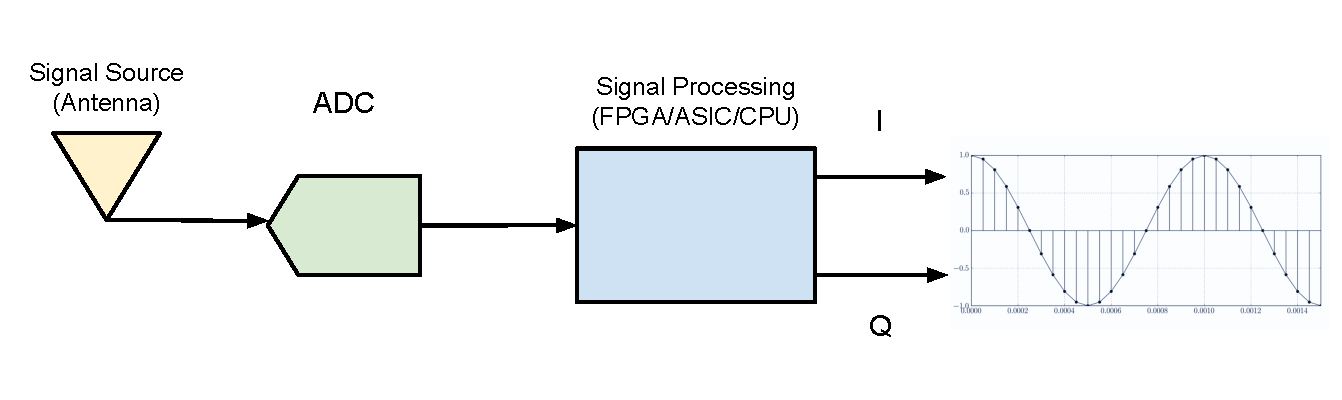
\includegraphics[width=\textwidth]{Images/SDR_Ideal_block.pdf}
\isucaption{An ideal software defined radiometer}
\label{ideal_sdr}
\end{figure}
}

A SDR allows can perform certain hardware functions, such as filtering, in the digital domain and is then defined by software.  Since the software is now processing the signal, it can rapidly change what functions are executed on the signal by changing the software.  This gives SDRs a high amount of flexibility because components that were normally done in hardware can now be done in software.  They can also be changed by simply uploading new software or firmware to the system.  This is a cost benefit as certain components are no longer needed and changes made in software do not require additional hardware to be added, deleted or changed.

A more realistic software defined radio is shown in figure \ref{prac_sdr}.  There are two items added to this software defined radio.  Amplification of the signal or gain is added to improve the sensitivity of the SDR.  A mixer can often be used to down-convert a high frequency RF signal to a lower frequency signal in order to use a less expensive analog to digital converter.  If however, the original frequency is already within the range of the analog to digital converter, the mixer may be omitted.  

%An ideal software defined receiver simply has an antenna connected to an analog to digital converter which sends information to a processing unit such as a Field Programmable Gate Array (FPGA) or computer.  For a transmitter, we reverse it and use a digital to analog converter to produce the correct waveform which is then transmitted by the antenna.  In reality, SDRs require some additional hardware to make a viable working transceiver.  Amplification is still required to amplify the incoming signal and to amplify the signal going to the antenna.  Some SDRs also use a mixing stage to move a high frequency signal to a lower frequency signal.  This allows for less expensive analog to digital and digital to analog converters to be used.  

{\begin{figure}[h!tb] 
\centering
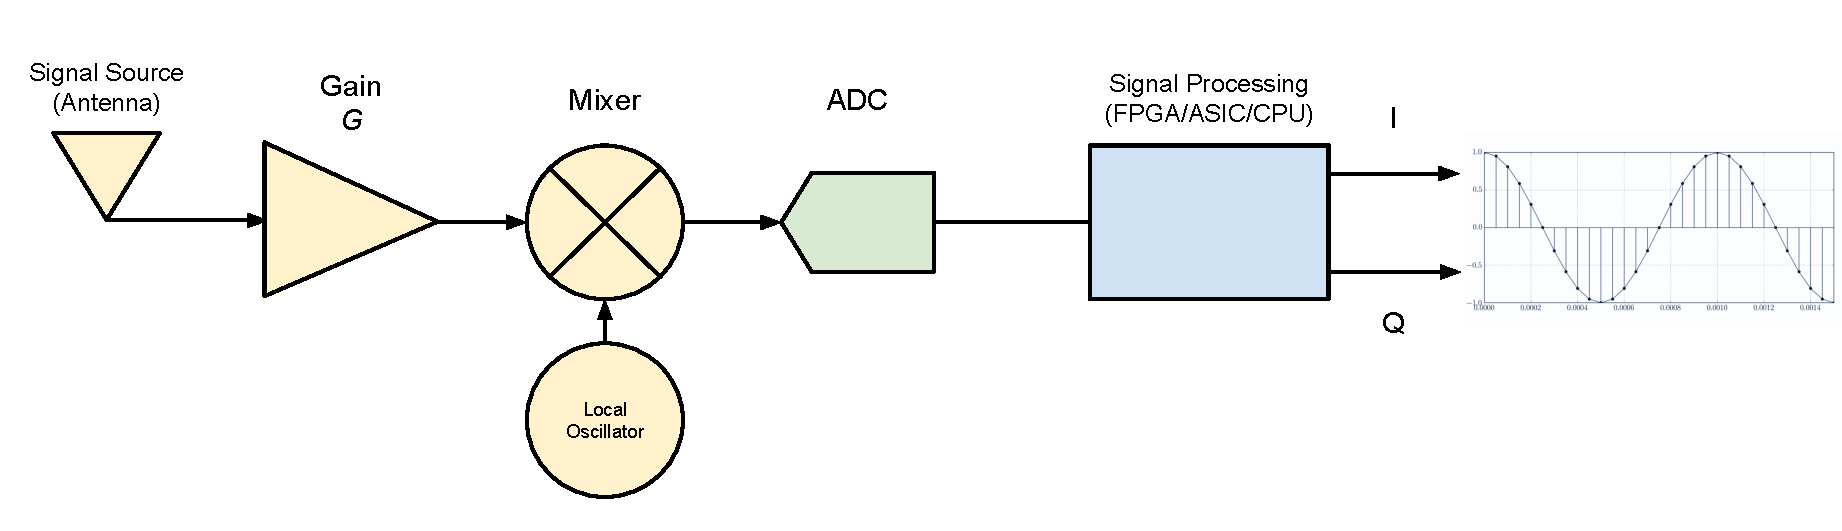
\includegraphics[width=\textwidth]{Images/SDR_Prac_block.pdf}
\isucaption{A typical software defined radiometer}
\label{prac_sdr}
\end{figure}
}

\emph{Software Defined Radio Applications.}  Software Defined Radios (SDRs) are used for a variety of applications, but their primary application has been in the area of communications.  Some examples of these applications include:  mobile communications, wireless local area networks, personal area networks and digital broadcast.  They appeal to applications where having the ability to change a modulation scheme or filter on the fly is desirable.  In these areas, SDRs often outperform traditional hardware-only radios in their ability to easily change their operations by changing the software.  

Early SDRs were expensive due to the high costs in the analog to digital converters (ADCs) needed and the high speed Field Programmable Gate Arrays (FPGA) used.  In recent years, the cost of SDRs have decreased due to the cost of these key components decreasing.  Even though the cost has gone down, the performance of SDRs have increased.  This has led to developments in using SDRs in new and different ways[\cite{jondral2005software}].


%But this is the strength of a software defined radio, it is capable of performing all of these operations and can be adapted to new ones by simply updating the software that defines it.

\section{Software Defined Radio Development Platform} \label{SDR_platform}
This section will discuss the development platform used to develop a software defined radiometer.  The hardware and software tools used are off the shelf tools used for software defined radio development.  This section will examine the hardware platform used and discusses the software platform used.  

%The work of this thesis is to use an off the shelf software defined radio (SDR) to perform the same operation or better of a traditional analog radiometer.  Using a SDR radio also means that we are able to be more flexible in how the radiometer performs, is capable of frequency agility and adapting to changing conditions such as interference.  Using a software defined radio also allows for implementation of different radiometer types such as a correlation radiometer or a polarimetric radiometer that uses Stokes parameters [\cite{Wang}].  Normally, these require changes to hardware, but all of these types of radiometers can be implemented in software increasing the flexibility of the system.  

\subsection{Hardware Platform}
The hardware platform selected for this work is the Ettus Research Group N200 SDR and can be seen in figure \ref{N200}.  The N200 has the following features that made it desirable for our specific application:

\begin{itemize}
\item Dual 14-bit ADC,
\item 25 MHz bandwidth per channel,
\item Modular daughter-board system for RF front end.
\end{itemize}

The flexible architecture and the ability of the N200 to handle large amounts of bandwidth made this hardware ideal for the software defined radio radiometer work done in this thesis.

{\begin{figure}[h!tb] 
\centering
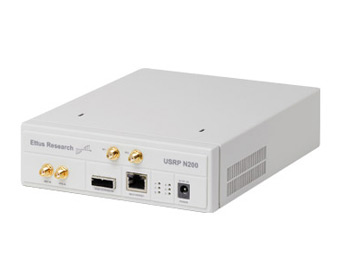
\includegraphics{Images/n200}
\isucaption{The USRP N200 from Ettus Research (Image from Ettus Research Website - www.ettus.com)}
\label{N200}
\end{figure}
}

When selecting the hardware for this thesis, the requirements defined in chapter \ref{ch:implementation}, section \ref{requirements} were examined in detail.  The bandwidth requirement was a deciding factor in the hardware selected.  The requirement stated that a minimum of 20 MHz needs to be processed by the SDR.  The N200 selected is capable of 25 MHz per channel and this met the requirement.  The 14-bit ADC was not a defined requirement, but it does allow the ability to accurately record the signal with a high level of resolution.  

The N200 utilizes a flexible architecture through the use of daughter-boards for a variety of RF systems.  Figure \ref{N200_block} shows the overall architecture of the N200 SDR.  This daughter board directly receive the RF signal and then outputs the analog I and Q signals that are then sampled by the N200 A/D converter for reception or receives the I and Q values from the N200 D/A converter for transmission. 

{\begin{figure}[h!tb] 
\centering
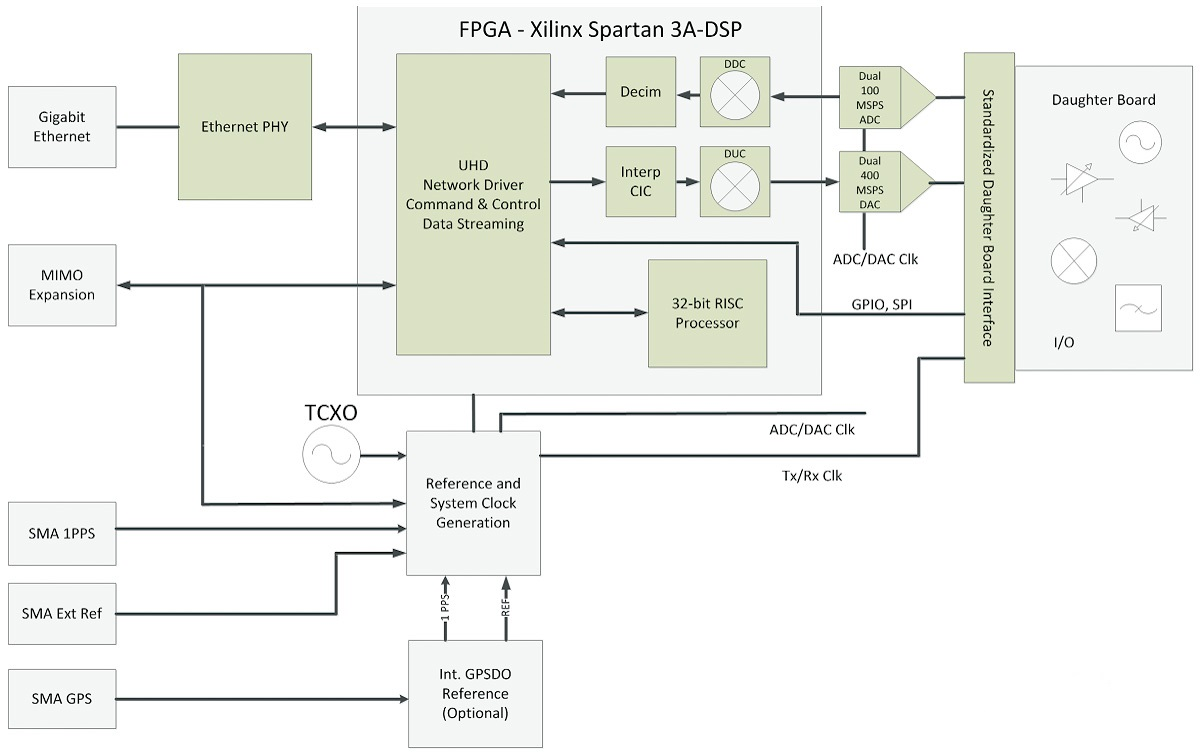
\includegraphics[width=14cm]{Images/n200_block_edited}
\isucaption{A block diagram of the Ettus N200 SDR. (Image from Ettus Research Website - www.ettus.com)}
\label{N200_block}
\end{figure}
}

%The requirements outlined above was the guiding factor in selecting the N200 SDR for our hardware platform.  These reasons, and the fact that this hardware is well supported by GNURadio, lead to using this for the work in this thesis.
%While not a defined requirement, it was indicated by Dr. Brian Hornbuckle that it would be ideal to look at two signals at the same time.  The N200 is able to have up to two daughter boards installed.

\emph{The DBSRX2 Receiver.}  The daughter board selected is the DBSRX2 daughter board shown in figure \ref{dbsrx2}.  This daughter board is a receive only and operates between 800 MHz and 2400 MHz.  A requirement for this system is operation between 1400 MHz and 1425 MHz, and this daughter board meets those requirements.  

{\begin{figure}[h!tb] 
\centering
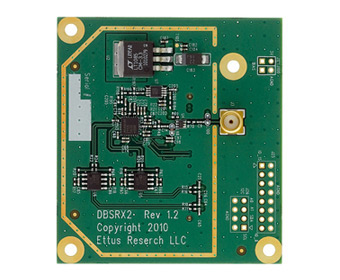
\includegraphics{Images/dbsrx2.jpg}
\isucaption{The DBSRX2 daughter board from Ettus Research (Image from Ettus Research Website - www.ettus.com)}
\label{dbsrx2}
\end{figure}
}

The DBSRX2 has all of the RF hardware needed to process our RF signal.  This includes a programmable gain amplifier, a direct-conversion converter, a mixer and finally a band pass filter that can be seen in figure \ref{dbsrx2_block}.  First the signal is amplified through a Programmable Gain Amplifier (PGA).  This PGA is accessible from the software and can be configured by the software.  Next the signal goes into a direct-conversion integrated circuit, a Maxim 2112.  This integrated circuit directly converts the RF signal to analog I and Q values and uses an integrated mixer and bandpass filter.

{\begin{figure}[h!tb] 
\centering
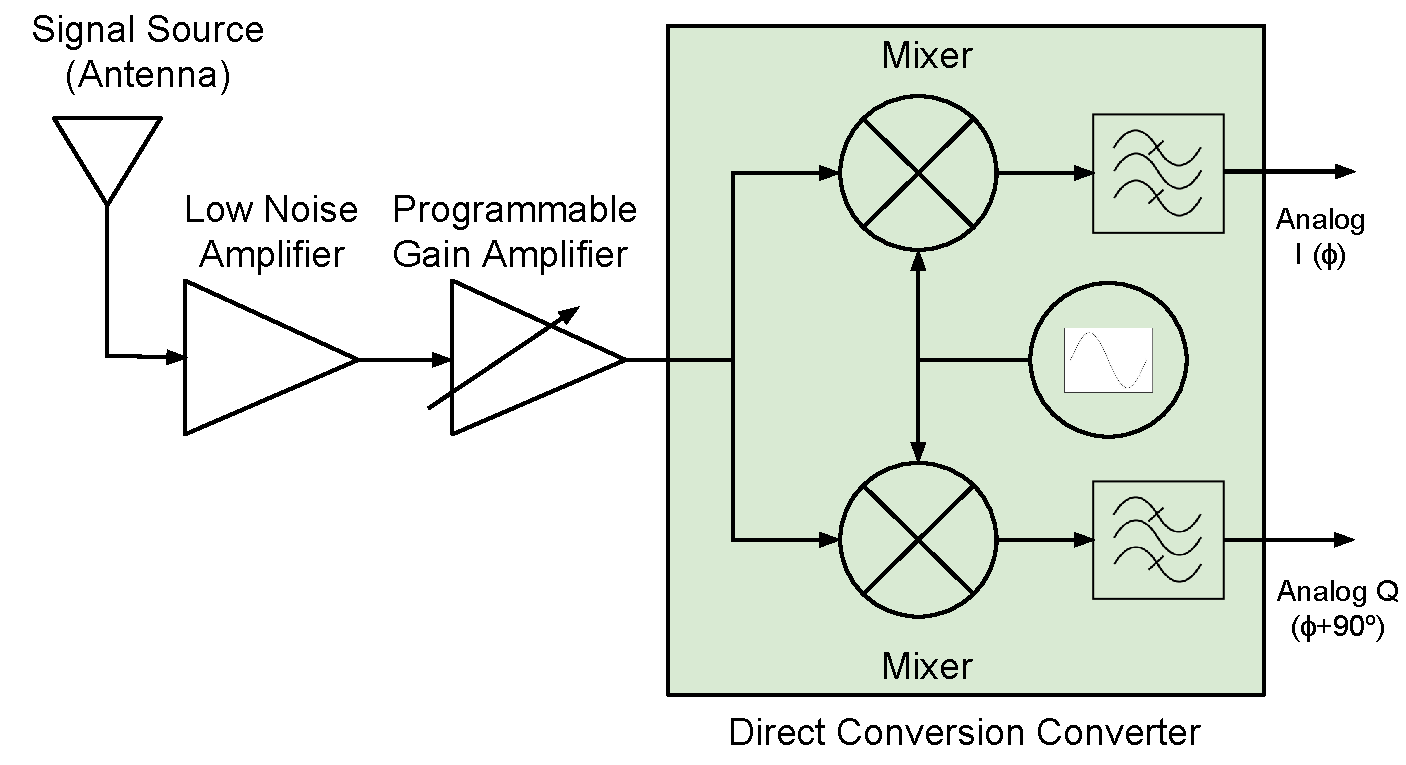
\includegraphics[width=\textwidth]{Images/DBSRX2_block.pdf}
\isucaption{Block diagram of the DBSRX2 daughter board.}
\label{dbsrx2_block}
\end{figure}
}

%{\begin{figure}[h!tb] 
%\centering
%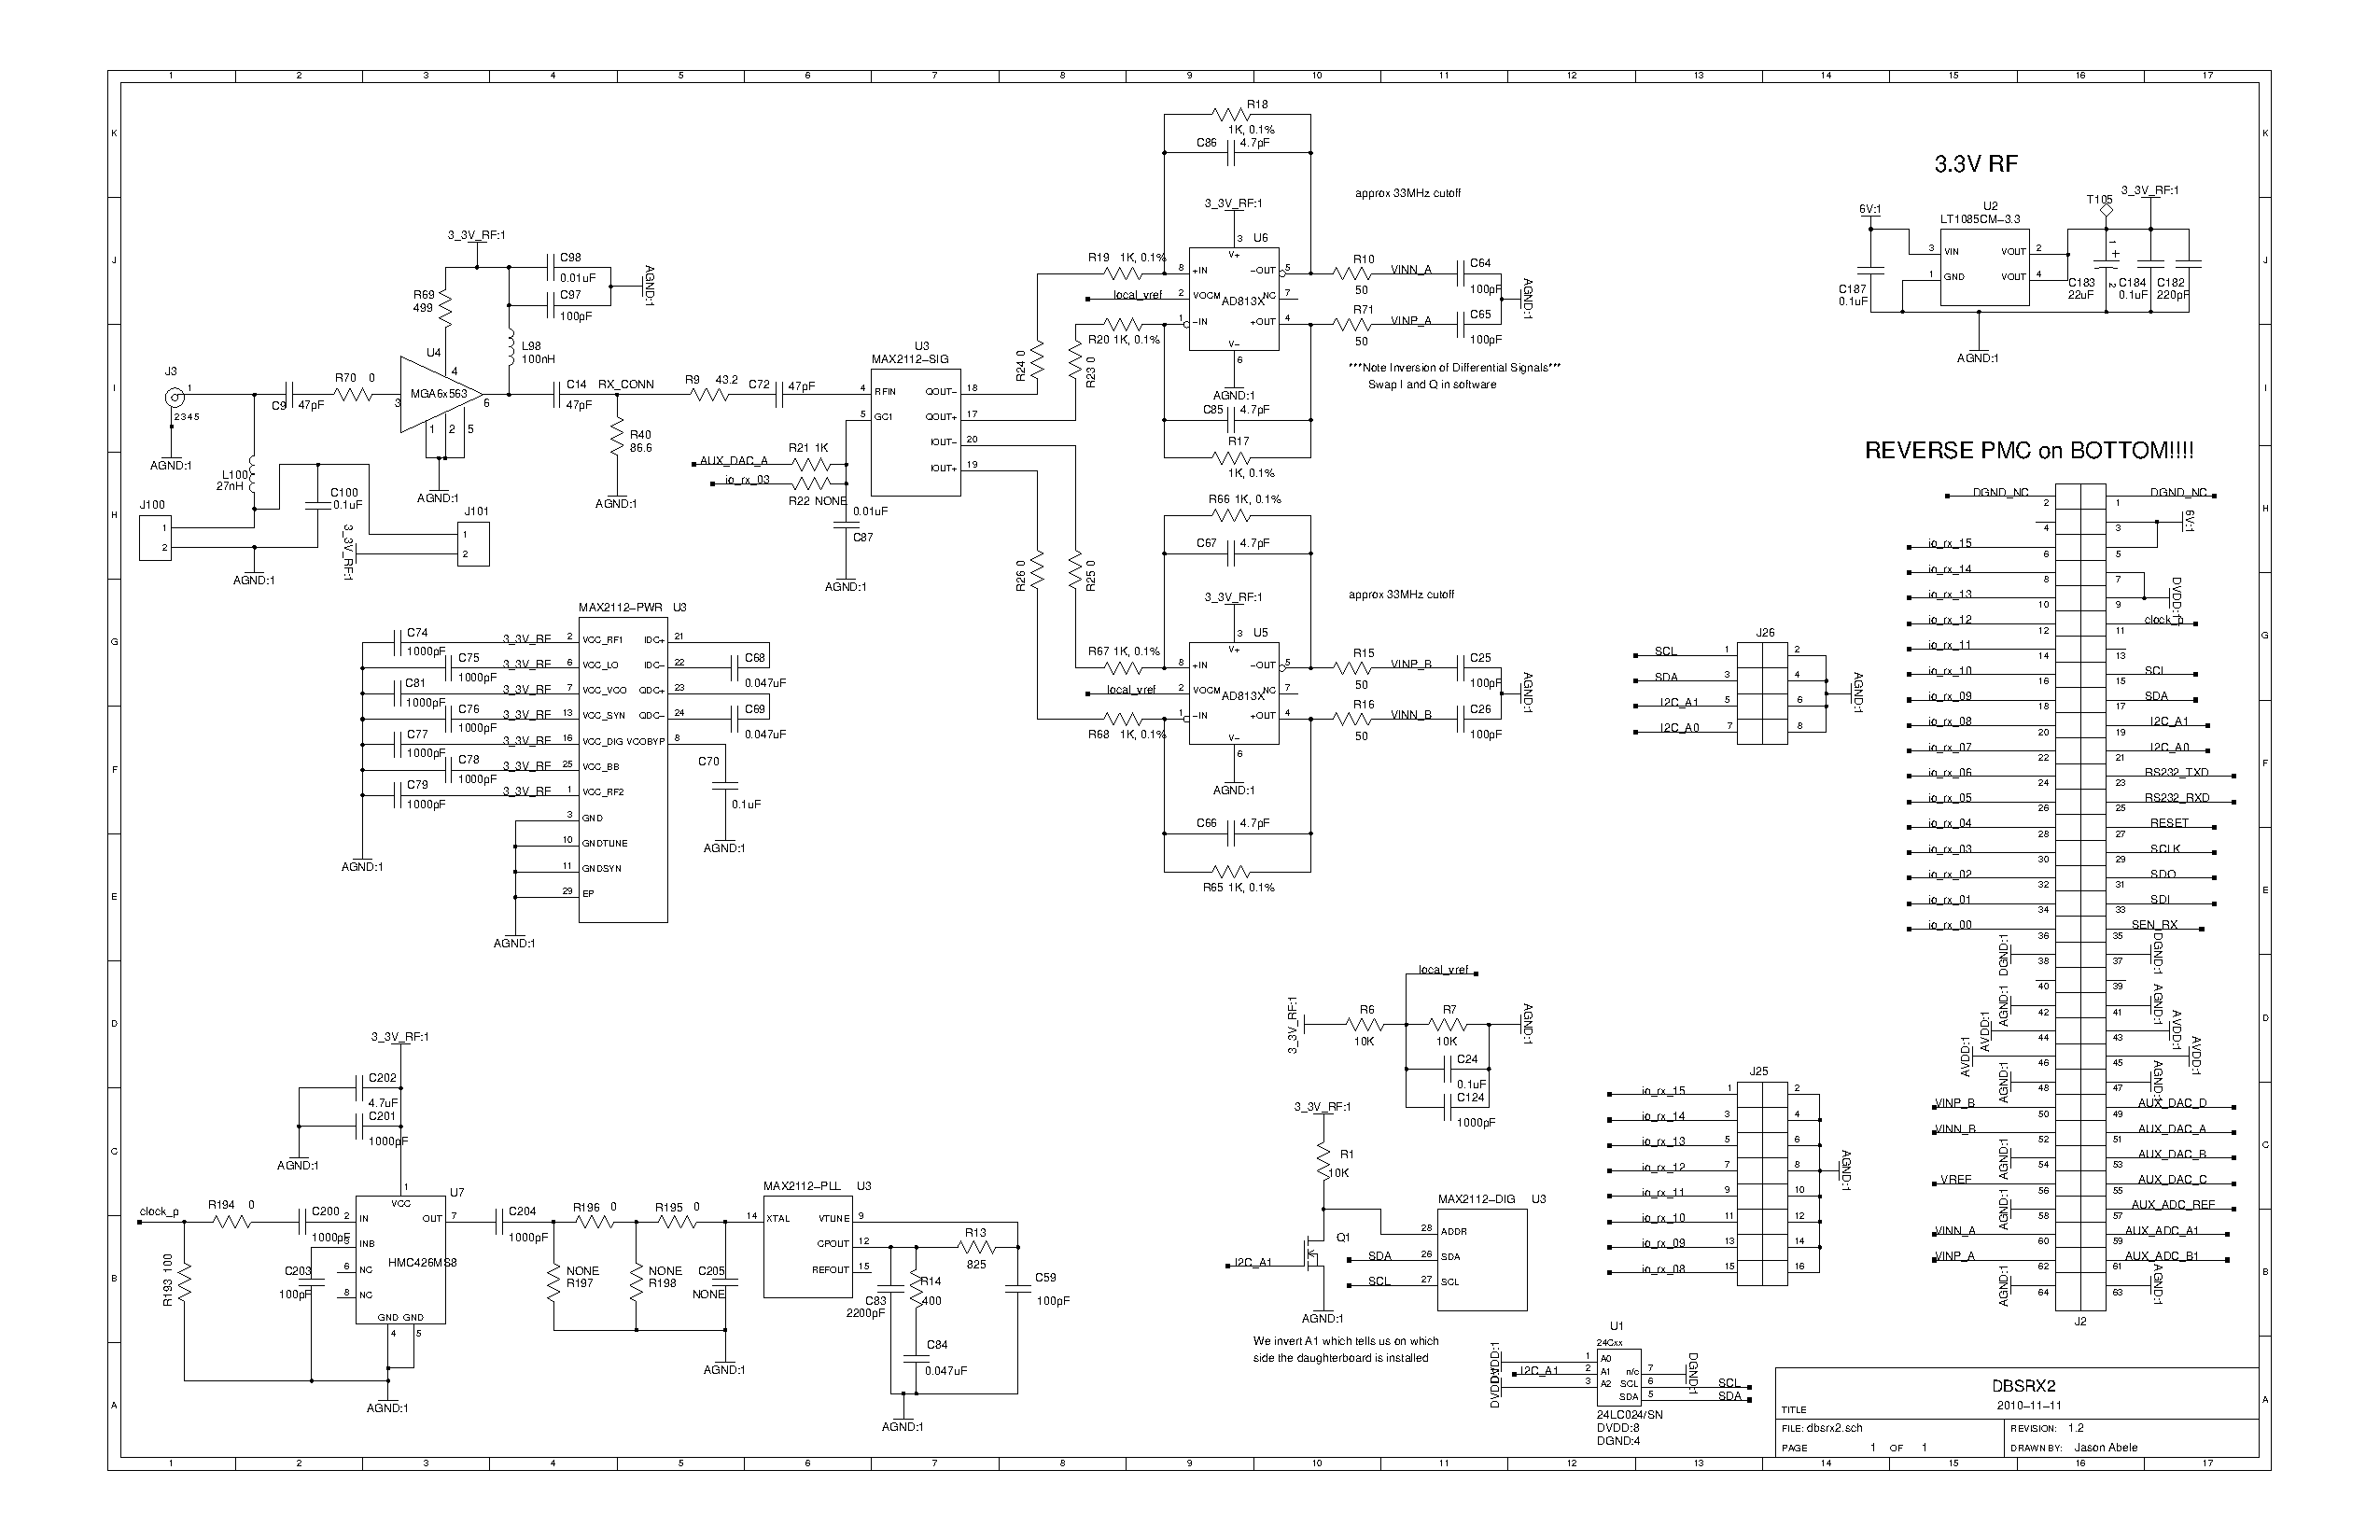
\includegraphics[width=\textwidth]{Images/dbsrx2.pdf}
%\isucaption{The DBSRX2 Schematic (Image from Ettus Research Website - www.ettus.com)}
%\label{dbsrx2_sch}
%\end{figure}
%}

These analog I and Q values are then sent to the the analog to digital converter to be digitized.  The IQ values are differential signals to minimize interference due to noise.  Once digitized, the digital I and Q values are sent to the FPGA to be processed and then sent to the computer for signal processing.

%Since we are using the DBSRX2 after the LNAs that are already in use, the noise temperature added by the DBSRX2 will be small.  The DBSRX2 adds approximately 1.05 dB to the overall noise factor of the system.

\subsection{Software Platform} \label{software_platform}

There are two pieces of software that are used with the software defined radio:  1) the firmware that is used in the FPGA of the N200 and 2) the software running on the host computer.  

The firmware provides low level processing of the signal so it can be sent to the software located on the computer.  It also provides a link for controlling key aspects of the software defined radio such as gain, bandwidth and the center frequency.  This firmware is already pre-loaded into the FPGA by Ettus Research and can be upgraded using tools provided by Ettus Research.

The software on the host computer is the software that provides the signal processing on the I/Q data.  For this task, GNURadio was selected.   GNUradio is an open source software designed for software defined radios.  It is also well supported by our hardware.  It also provides a GUI framework to create an interactive environment for the user.   

GNURadio uses a combination of Python and C++, where Python handles the high level interface and C++ is used as drivers and low level interface to the hardware.  This combination allows for a system that is easy to use, but still meets the demanding performance of handling large amounts of data. 

GNURadio also has a rapid development tool called GNURadio companion, or GRC.  GRC uses a simple to use graphical system to design and build radio components in software. An example of GRC is shown in figure \ref{N200_GRC}.

{\begin{figure}[h!tb] \centering
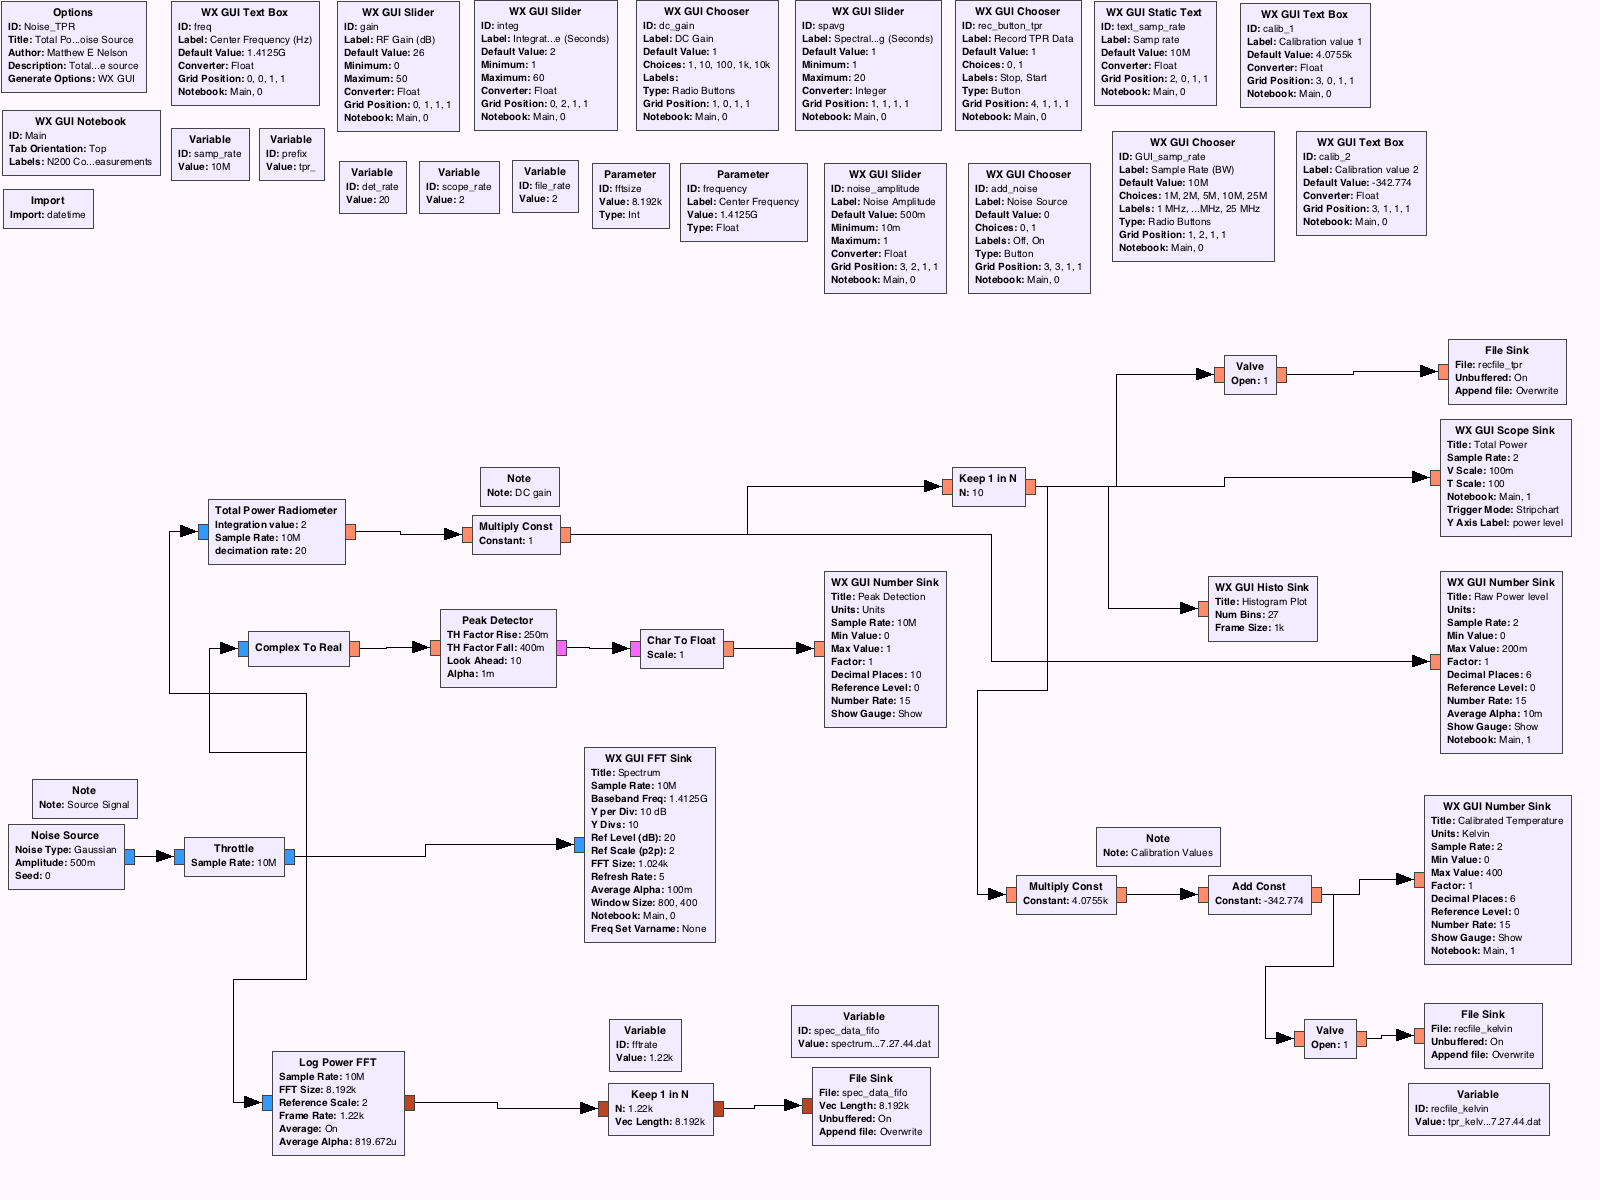
\includegraphics[width=\textwidth]{Images/noisesrc_radiometer.png}
\isucaption{A screenshot of the GNURadio Companion editor program.  Source:  GNURadio}
\label{N200_GRC}
\end{figure}
}

GNUradio Companion works by having the common functions, such as signal sources, signal processing and signal sinks, as blocks that can picked and placed on the screen.  Once placed, the blocks can be wired up, much like LabView, and the flow of data can be controlled in this fashion.  GNURadio Companion also includes blocks that allow for building a GUI interface.  This gives us tools for building a user interface to display data and control the software defined radio.

If a block does not exist, it is possible to create new blocks.  Because GNURadio uses Python, users can use this powerful and flexible language to build new blocks that can be imported into GRC.  

%Additional blocks can also be created using Python.  This allows the users to create other blocks and access other common Python libraries.  Each block is then defined in While GNURadio Companion provides most of the essential blocks used in most applications additional blocks can by added if needed.  This is done by using Python and the blocks in GNUradio Companion are simply blocks of Python code.  To compile a GNURadio Companion flow diagram, you simply run the sheet, which then generates the Python code that is then executed.   


With GNURadio and GNURadio Companion, a software defined radio can be rapidly built with little programming experience.  The excellent support of the hardware selected and the ease of use of this software made it ideal for our development tool for building the necessary software in our software defined radiometer.

%----------------------------------------------------------
% End of Chapter 3.  Anything below this is extra information

%The amount of noise that is generated by the object of interest is due to the thermal agitation of the charge carriers, usually the electrons, which is directly correlated to the physical temperature of the source[\cite{Nyquist1928thermal}].  This correlation is done as a noise temperature.  All objects emit this noise and the intensity will vary on multiple parameters and on what the source is.  One source that has current research at Iowa State University is in detecting soil moisture.  Numerous soil types can be observed including sandy types of soil[\cite{Liu}], The brighter or warmer the noise temperature is, the more RF noise that has been received which correlates to a drier soil.  The less RF noise power received the cooler the noise temperature and this indicates wetter soil area. Radiometers such as these are already in service on satellites such as the Soil Moisture and Ocean Salinity (SMOS) satellite launched by the European Space Agency (ESA) and are used by scientists to monitor the Earth's soil moisture and ocean salinity[[\cite{McMullan}][\cite{Hardy}]. 

%{\begin{figure}[h!tb] 
%\centering
%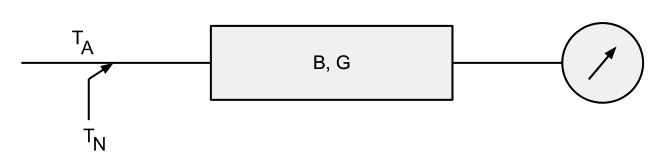
\includegraphics[width=\textwidth]{Images/radiometer_noise_added.png}
%\isucaption{A more realistic radiometer model}
%\label{noiserad}
%\end{figure}
%} 

%{\begin{figure}[h!tb] 
%\centering
%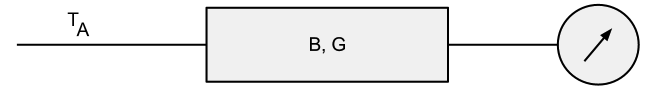
\includegraphics[width=\textwidth]{Images/simple_rad.png}
%\isucaption{The ideal radiometer block diagram}
%\label{simplerad}
%\end{figure}
%}

%Figure \ref{simplerad} shows us an ideal radiometer.  That is a radiometer that has an input from the antenna, $T_{A}$, a known bandwidth denoted as $B$ or $\beta$ and a known gain denoted as $G$.  At the end of the block is the detector, which measures the power from the radiometer.

%Only a certain selection of the radio spectrum is observed by the radiometer and this is the bandwidth of the radiometer.  In our scenario, we center around 1.4125 GHz.  There is a reason why 1.4125 GHz is selected and that is from 1.4000 to 1.4250 GHz is protected internationally to be as radio frequency interference free as possible.  This reduces interference from outside sources such as transmitters that can interfere with the operation of the radiometer.  

%The power coming from the antenna is the combination of the following items:

%\begin{enumerate}
%\item Gain or $G$ of the system,
%\item Bandwidth or $\beta$ of the system,
%\item Signal source or $T_{A}$.
%\end{enumerate}

%These specifications had a large impact on the selection of the N200 for this application.  Specifically the 14-bit ADC, the 50 MS/s and the modular daughter-board system were the largest factors in the decision to use the N200 SDR.  Further explanation on these specifications are explained in the following sections.

%\emph{14-bit ADC.}  The analog to digital converters (ADC) allow us to take the analog I and Q values from the daughter boards and digitize this information.  Once digitized, we can now work with the signal both on the on-board FPGA board or stream it to the computer so that our software can manipulate the signal.  In radiometry, we are primarily looking at the overall power of the signal and this does not require us to accurately recreate the signal.  However, as will discuss later there are times were we do want frequency information and having an accurate frequency representation of the signal will then be an important factor.

%\emph{50 MS/s Bandwidth.}  The N200 is capable of working with up to 100 MS/s signal and can stream up to 50 MS/s through the Gigabit Ethernet connection.  The N200 also has the ability to have up to 2 daughter boards installed.  If we assume each will have up to a 20 MHz signal, this means up to 40 MS/s of data will be required.  This means that the N200 meets and can exceed the bandwidth requirements that we were looking for.  In addition, the FPGA on the N200 is capable of working with up to 100 MS/s, so there is room in handling additional bandwidth by using the on board FPGA to process the signal.

%The daughter board selected is the DBSRX2 card as this card is receive only and operates between 800 MHz and 2.4 GHz.  The DBSRX2 also has built in amplification that is adjustable through software.

%{\begin{figure}[h!tb] 
%\centering
%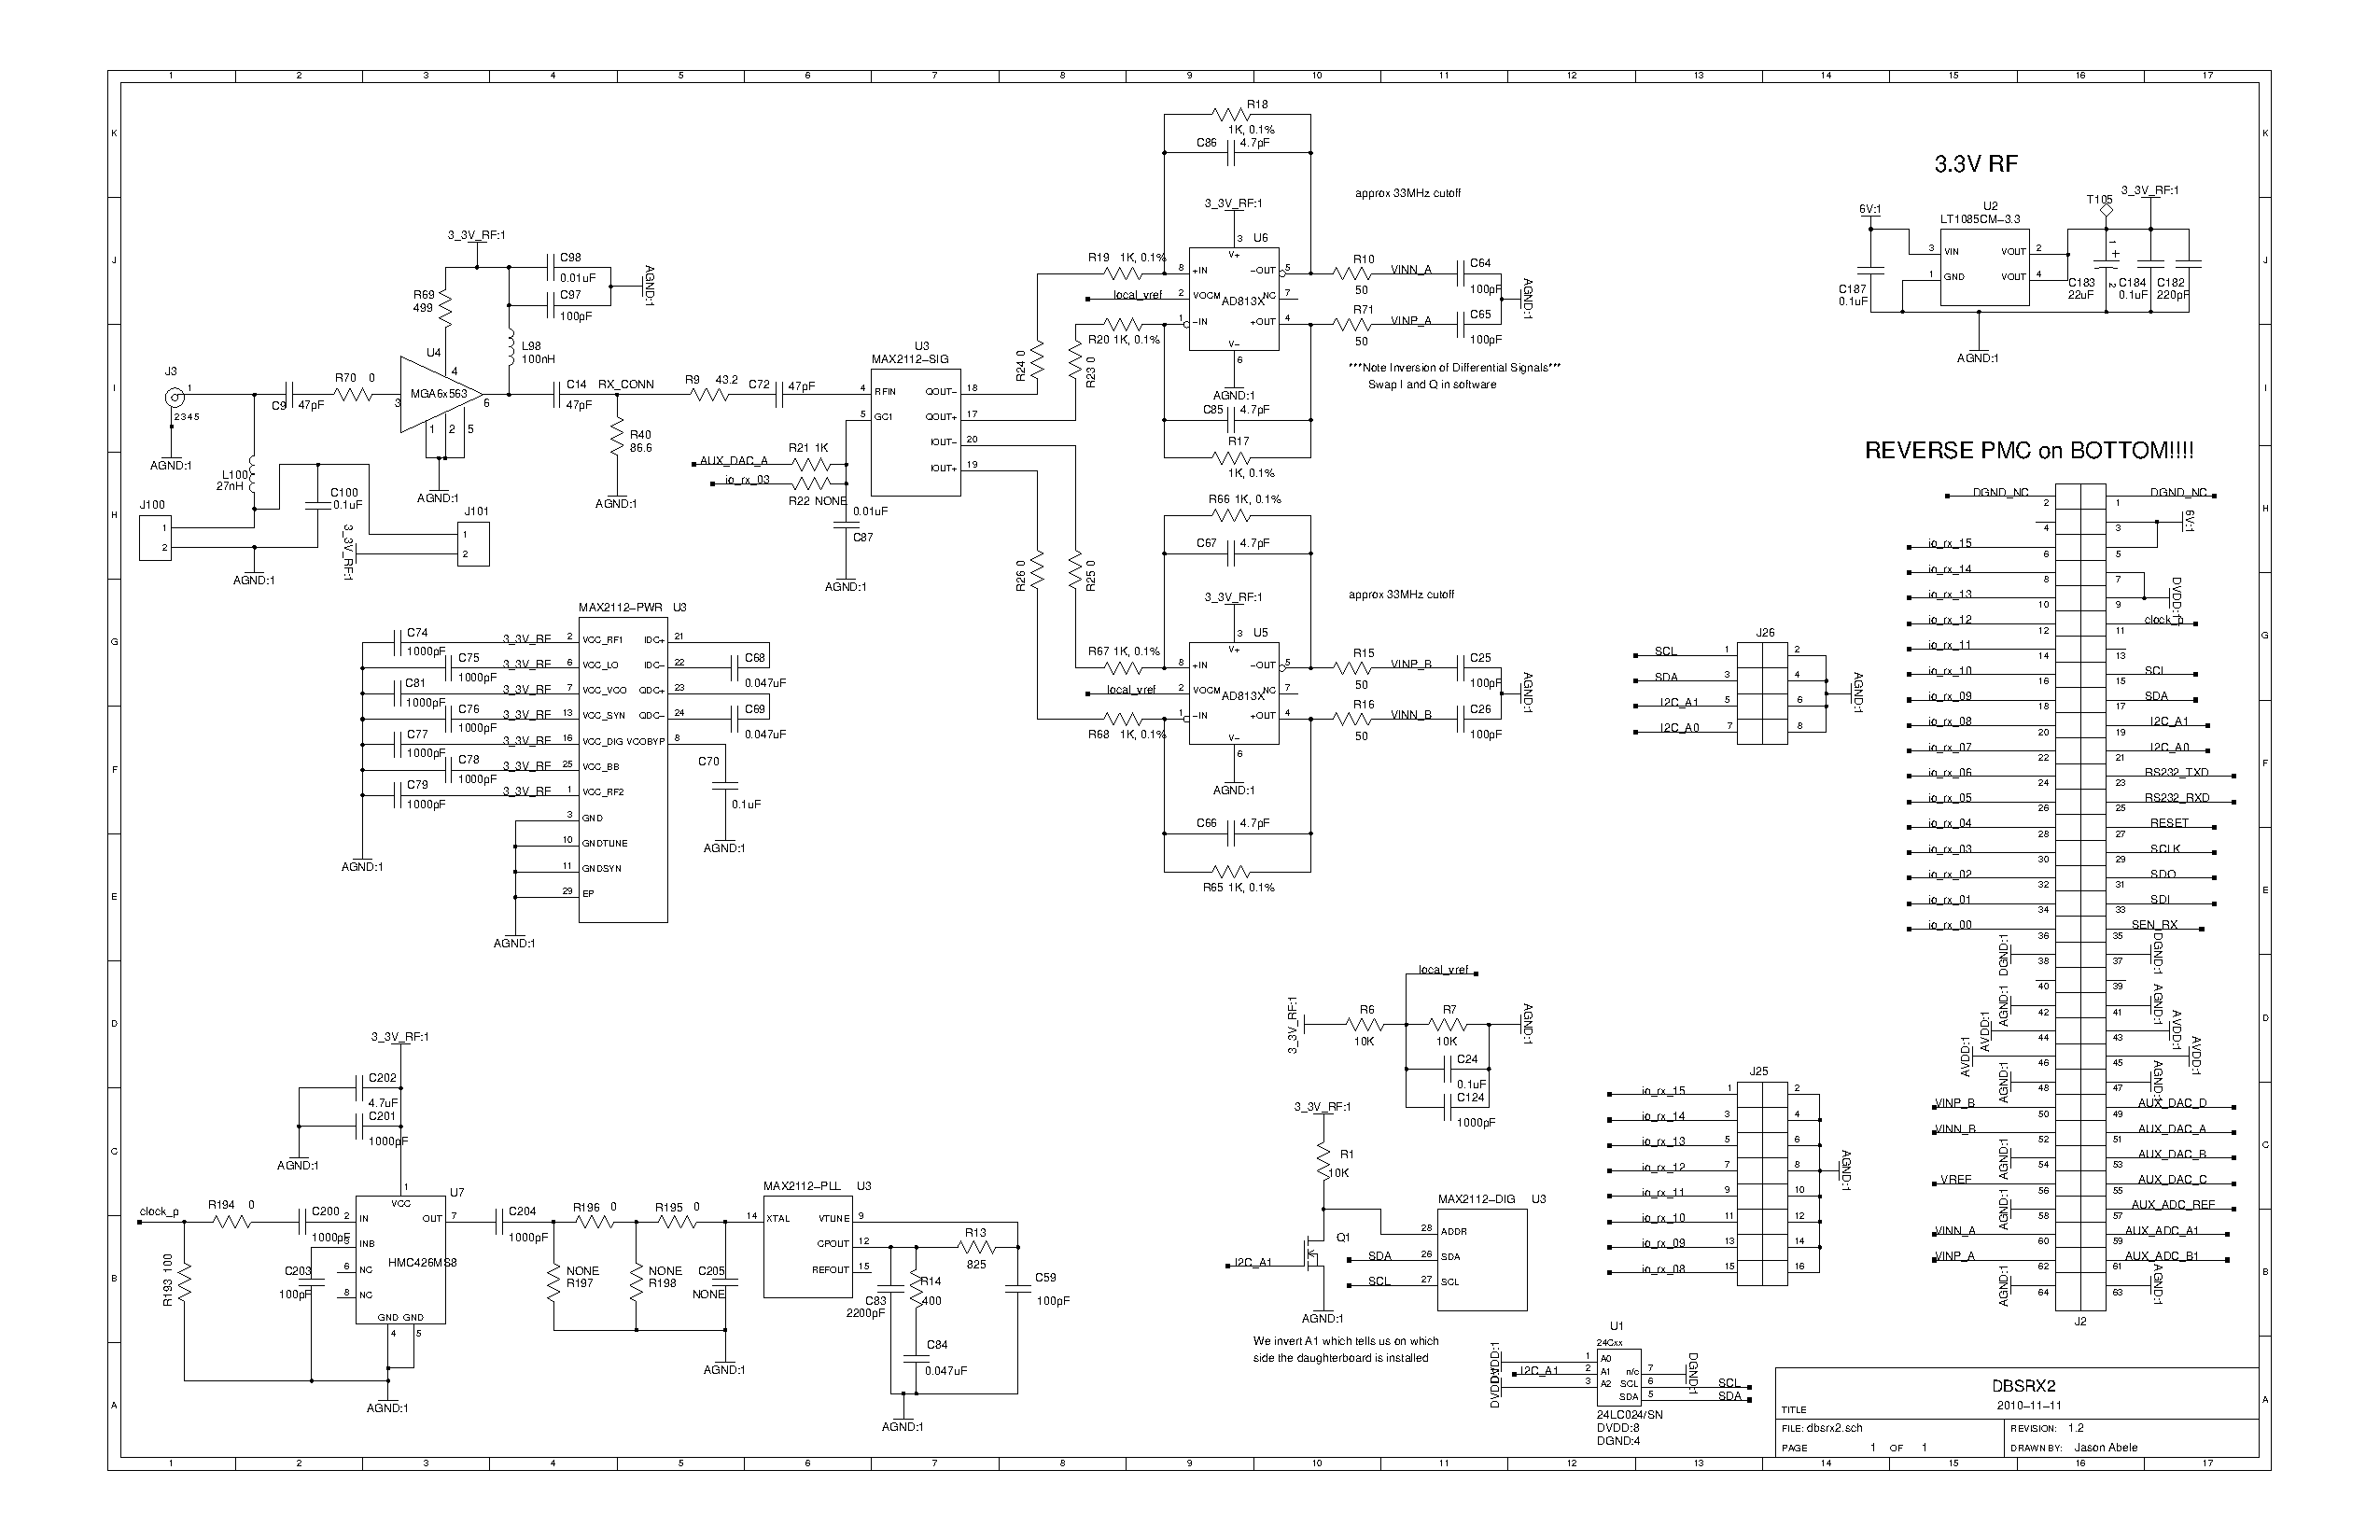
\includegraphics[width=\textwidth]{Images/dbsrx2.pdf}
%\isucaption{The DBSRX2 Schematic (Image from Ettus Research Website - www.ettus.com)}
%\label{dbsrx2_sch}
%\end{figure}
%}

%GNURadio  and GRC is written in Python, which allows for easy modification and access to additional tools that can be used with GNURadio.  While most of GNURadio is written in Python, C is used for any of the low level drivers and interface to the hardware.  This is done to optimize speed and performance of GNURadio.

%GNURadio fills in the software side of the software defined radio.  Although there is firmware that runs on the FPGA in the N200, this firmware is designed to communicate with a host PC.  It is this software that does most of the work by doing the calculations that apply to the signal.  The FPGA simply sends the raw IQ data to the host PC, which then performs the necessary math functions.  Again, the reason why software defined radios are desirable is the ability to change the behavior of the radio quickly.  In our scenario we can change functionality by simply loading a new software program in the host PC.  

%This functionality is ideal for communication type of radios where different modulation schemes and encoding and decoding methods can easily be changed out.  However, in a radiometer we are not interested in this aspect of the SDR.  However, one functionality is available that can be valuable for a radiometer, and that is with filtering.  Although we often use frequencies that should be free from interference, this is not always what happens in the real world.  Interference can and often does still occur, even in these protected frequencies.  With the SDR, we are able to quickly adapt to changing conditions by moving the frequency, changing our bandwidth and even filter out an offending signal.  

%GNURadio was selected as it is an open source software platform.  GNURadio is licensed under the GPL license and has a strong community that continually updates the software.  It is also well supported by third parties such as Ettus Research Group, National Instruments and other SDR developers.  In addition, GNURadio has a strong set of tools that can be used to develop programs that run under GNURadio.  Tools such as the GNURadio Companion (GRC) allows for an easy to use GUI to develop code for GNURadio.  GNURadio is also written in Python, which allows for easy modification and access to additional tools that can be used with GNURadio. 

%{\begin{figure}[h!tb] 
%\centering
%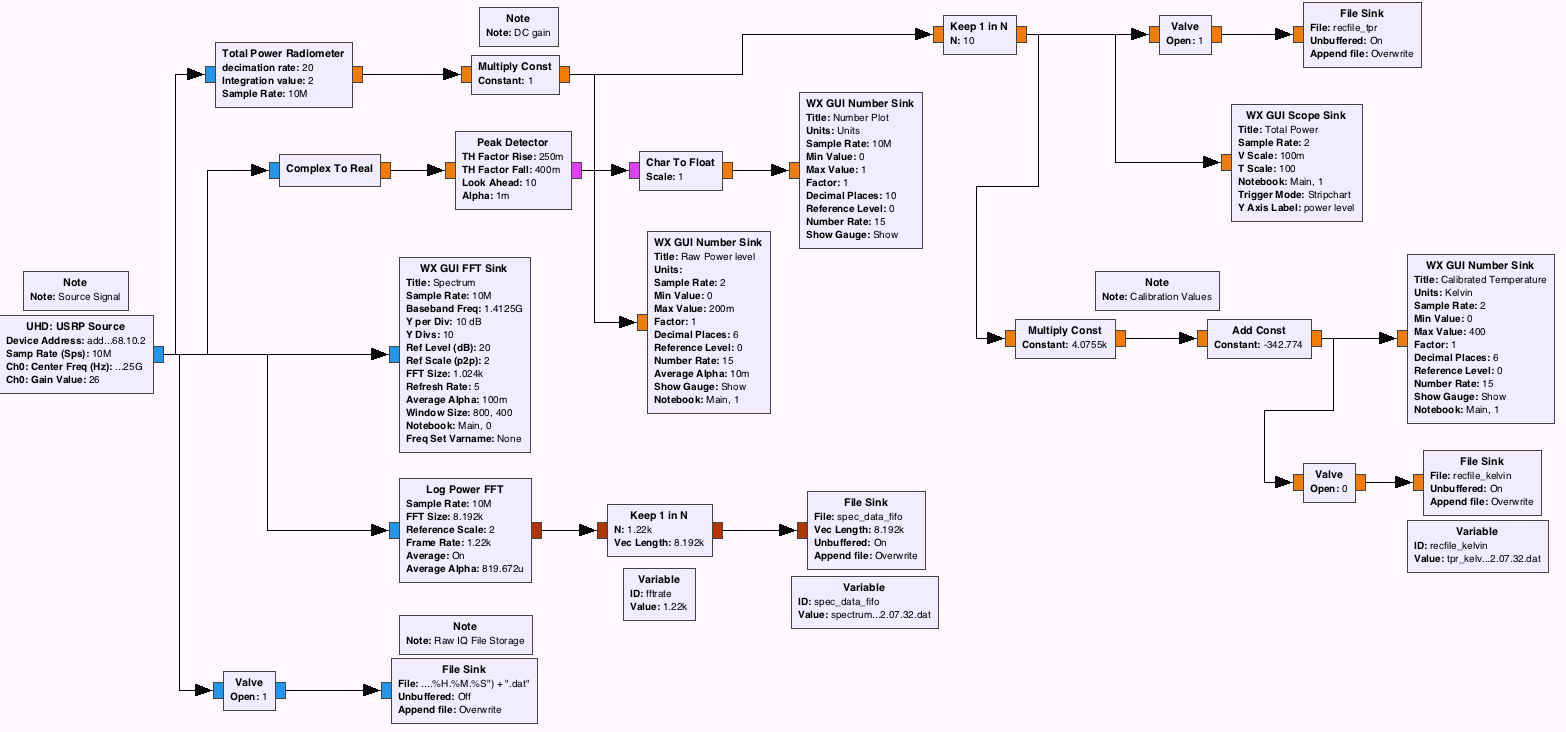
\includegraphics[width=17cm]{Images/N200_radiometer_grc.png}
%\isucaption{Screenshot of the GNURadio Companion editor and the N200 Radiometer block diagram used in the author's experiments}
%\label{N200_GRC}
%\end{figure}
%}
 